\documentclass[12pt,a4paper]{report}

% Encodage et langue
\usepackage[utf8]{inputenc}
\usepackage[T1]{fontenc}
\usepackage[french]{babel}
\usepackage[absolute,overlay]{textpos}


% Mise en page
\usepackage{geometry}
\geometry{left=2.5cm,right=2.5cm,top=2.5cm,bottom=2.5cm}
\usepackage{setspace}
\onehalfspacing

% En-têtes/pieds de page
\usepackage{fancyhdr}
\fancypagestyle{plain}{%
  \fancyhf{} % vide
  \lhead{Serpent}
  \rhead{UNC - 2025}
  \cfoot{\thepage}
}


% Maths et figures
\usepackage{amsmath, amssymb}
\usepackage{graphicx}
\usepackage{hyperref}


% Pour la bibliographie simple
\usepackage{url}

% <<< ADD THE FIX HERE >>>
\usepackage{etoolbox}
\makeatletter
\patchcmd{\@makeschapterhead}
  {\vspace*{50\p@}}{\vspace*{10pt}}{}{}
\patchcmd{\@makeschapterhead}
  {\vskip 40\p@}{\vspace{15pt}}{}{}
\makeatother
% <<< END FIX >>>

\renewcommand{\thesection}{\arabic{section}}


\begin{document}

% Page de garde
\begin{titlepage}

    % --- Logo en haut à droite ---
    \begin{textblock*}{5cm}(15cm,0.5cm)
        
\includegraphics[width=5cm]{assets/logo.png} 
    \end{textblock*}

    % --- Titre justifié et limité ---
    \noindent
    \begin{minipage}{13cm}
        \raggedright
        {\scshape\Huge \textbf{Algorithme de chiffrement par bloc : Serpent} \par}
    \end{minipage}

    \vspace{0.cm}

    \rule{\linewidth}{0.4pt}
    
    \vspace{0.1cm}

    \centering
    {\Large Rapport\par}

    \vspace{1.5cm}
    {\large NGUYEN Alexandre - MILLOT Nathan\par}

    \vspace{4cm}
    % --- Image du sujet ---
    \begin{center}
        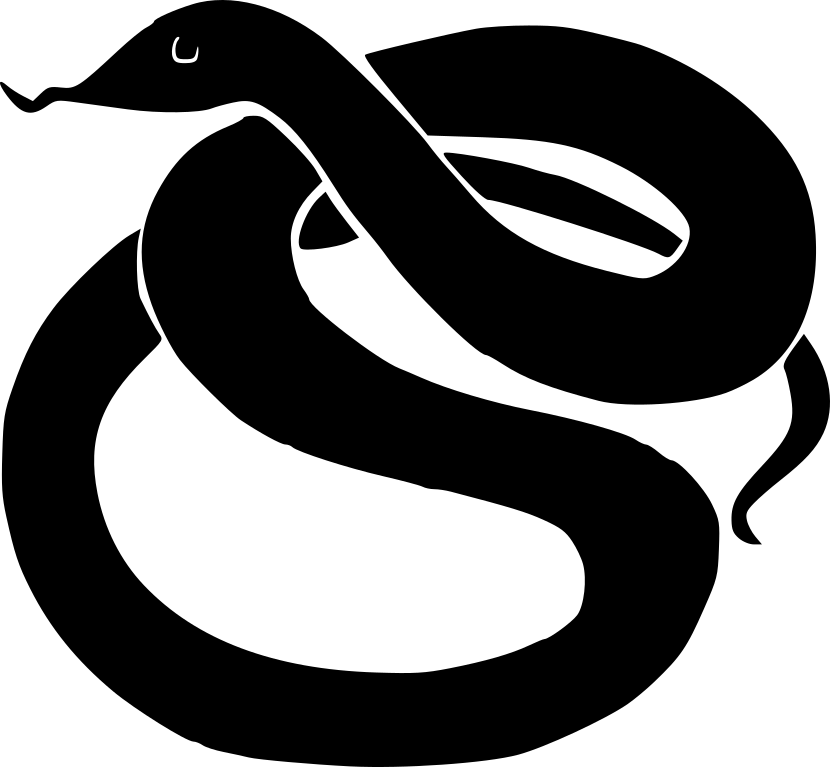
\includegraphics[width=0.5\linewidth]{assets/serpent.png}
    \end{center}

    \vspace{2.5cm}
    {\large Licence Informatique TREC 7  Semestre 6 \par}
   
    \vspace{1cm}
    {\large Date : \today \par}

\end{titlepage}

\tableofcontents
\newpage

\chapter*{Espaces de définition}
\addcontentsline{toc}{chapter}{Espaces de définition}

\section{Messages en clair et chiffrés}
L’algorithme Serpent est un chiffrement par bloc avec :
\begin{itemize}
    \item Espace des messages en clair $M = \{0,1\}^{128}$ ;
    \item Espace des messages chiffrés $C = \{0,1\}^{128}$.
\end{itemize}
Chaque bloc est donc constitué de 128 bits.

\section{Clés}
L’espace des clés dépend de la taille choisie :
\begin{itemize}
    \item $K = \{0,1\}^{128}$ ;
    \item $K = \{0,1\}^{192}$ ;
    \item $K = \{0,1\}^{256}$.
\end{itemize}
En pratique, Serpent est défini pour ces trois tailles de clé.

\chapter*{Description du schéma Serpent}
\addcontentsline{toc}{chapter}{Description du schéma Serpent}

\setcounter{section}{0}

\section{Structure générale}
Serpent est basé sur un \textbf{réseau de substitution-permutation (SPN)}.  
Il comporte 32 rondes successives :
\begin{enumerate}
    \item Ajout de sous-clé (XOR avec la sous-clé de ronde) ;
    \item Substitution via une des 8 S-boxes (non-linéarité) ;
    \item Transformation linéaire (permutation de bits).
\end{enumerate}

\begin{figure}[h]
    \centering
    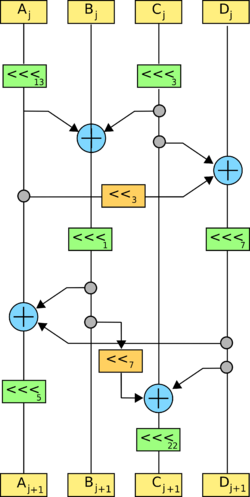
\includegraphics[width=0.4\textwidth]{assets/serpent-global.png}
    \caption{Schéma général de Serpent}
\end{figure}

\section{Sous-fonctions}

\subsection{Génération de sous-clés}
À partir de la clé initiale, Serpent dérive 33 sous-clés de 128 bits chacune, notées $K_0, K_1, \dots, K_{32}$.

\subsection{Substitution (S-boxes)}
Huit S-boxes différentes sont utilisées, notées $S_0, \dots, S_7$.  
Elles transforment des blocs de 4 bits en 4 bits, et sont choisies de manière cyclique au fil des rondes.

\subsection{Transformation linéaire}
Chaque ronde applique une permutation fixe des bits pour assurer une bonne diffusion.

\subsection{Dernière ronde}
La dernière ronde est légèrement différente : après la substitution, il n’y a pas de transformation linéaire, seulement l’ajout de sous-clé.

\chapter*{Exemple d’application}
\addcontentsline{toc}{chapter}{Exemple d'application}

Un cas concret d’utilisation de Serpent est son intégration dans certains logiciels de chiffrement comme \textbf{TrueCrypt} (ancien logiciel de chiffrement de disque), où il était proposé comme alternative à AES.  
Ce type d’application illustre bien l’usage de Serpent dans la protection des données sensibles stockées localement.

\chapter*{Sécurité et limites}
\addcontentsline{toc}{chapter}{Sécurité et limites}

\setcounter{section}{0}

\section{Résistance aux attaques}
Serpent a été conçu avec une marge de sécurité très élevée :
\begin{itemize}
    \item Résistant à la cryptanalyse différentielle et linéaire ;
    \item Résistant aux attaques par clé liée.
\end{itemize}
Ses 32 rondes sont considérées comme surdimensionnées par rapport au minimum nécessaire (16–24 rondes auraient suffi).

\section{Limites actuelles}

Malgré sa robustesse, Serpent n’a pas été choisi comme AES en raison de sa relative lenteur par rapport à Rijndael (AES).  
Aujourd’hui, il est toujours considéré comme sûr, mais il est moins utilisé que AES ou ChaCha20, qui sont devenus les standards de fait.

\chapter*{Conclusion}
\addcontentsline{toc}{chapter}{Conclusion}

Serpent est un algorithme de chiffrement robuste et bien conçu, qui mise sur la prudence et la sécurité.  
S’il n’a pas été choisi comme AES, il demeure un chiffrement respecté, encore pertinent pour l’enseignement et certaines applications pratiques.

\end{document}